\documentclass[11pt,a4paper]{article}
\usepackage[utf8]{inputenc}
\usepackage[T1]{fontenc}
\usepackage{amsmath,amssymb,amsfonts}
\usepackage{geometry}
\geometry{a4paper, margin=0.75in, headheight=26pt, headsep=12pt}
\usepackage{lmodern}
\usepackage{xcolor}

% Custom Color Palette
\definecolor{primaryblue}{RGB}{13, 71, 161}    % Deep Blue #0D47A1
\definecolor{secondaryblue}{RGB}{25, 118, 210} % Medium Blue #1976D2
\definecolor{accentred}{RGB}{198, 40, 40}     % Dark Red #C62828
\definecolor{accentgreen}{RGB}{46, 125, 50}    % Dark Green #2E7D32
\definecolor{bglight}{RGB}{248, 249, 250}     % Soft Gray background
\definecolor{bordergrey}{RGB}{207, 216, 220}  % Slate border
\definecolor{darkslate}{RGB}{38, 50, 56}      % Dark slate text
\definecolor{goldyellow}{RGB}{230, 140, 0}    % Deep Gold

\usepackage{tcolorbox}

% Custom tcolorbox Callout Boxes
\newtcolorbox{defbox}[1][Definition]{%
  colback=primaryblue!6!white,
  colframe=primaryblue,
  fonttitle=\bfseries\color{white},
  title={Geographic Definition: #1},
  arc=4pt,
  boxrule=1.5pt,
  before skip=10pt,
  after skip=10pt
}

\newtcolorbox{keybox}[1][Key Concept]{%
  colback=accentred!6!white,
  colframe=accentred,
  fonttitle=\bfseries\color{white},
  title={Key Theoretical Concept: #1},
  arc=4pt,
  boxrule=1.5pt,
  before skip=10pt,
  after skip=10pt
}

\newtcolorbox{modelbox}[1][Geographic Model]{%
  colback=secondaryblue!6!white,
  colframe=secondaryblue,
  fonttitle=\bfseries\color{white},
  title={Geographic Model / Paradigm: #1},
  arc=4pt,
  boxrule=1.5pt,
  before skip=10pt,
  after skip=10pt
}

\newtcolorbox{casebox}[1][Tribal / Regional Case Study]{%
  colback=accentgreen!6!white,
  colframe=accentgreen,
  fonttitle=\bfseries\color{white},
  title={Case Study: #1},
  arc=4pt,
  boxrule=1.5pt,
  before skip=10pt,
  after skip=10pt
}

\newtcolorbox{exambox}[1][Exam Focus]{%
  colback=goldyellow!8!white,
  colframe=goldyellow!95!black,
  fonttitle=\bfseries\color{white},
  title={Exam Revision \& Model Answer Outline: #1},
  arc=4pt,
  boxrule=1.5pt,
  before skip=10pt,
  after skip=10pt
}

\usepackage{tikz}
\usetikzlibrary{arrows.meta, positioning, calc, shapes, patterns}

\usepackage{fancyhdr}
\pagestyle{fancy}
\fancyhf{}
\fancyhead[L]{\parbox[b]{0.65\textwidth}{\raggedright\small\color{darkslate}\bfseries GGRMN21: Human Geography}}
\fancyhead[R]{\small\color{primaryblue}\bfseries Minor (Sem 2) | sciqb.com}
\fancyfoot[L]{\sffamily\color{gray}\small Notes by Aryan Maurya (sciqb.com)}
\fancyfoot[C]{\thepage}
\fancyfoot[R]{\sffamily\color{secondaryblue}\small\bfseries\href{https://sciqb.com}{sciqb.com}}
\renewcommand{\headrulewidth}{0.6pt}

\fancypagestyle{plain}{%
  \fancyhf{}%
  \fancyfoot[L]{\sffamily\color{gray}\small Notes by Aryan Maurya (sciqb.com)}%
  \fancyfoot[C]{\thepage}%
  \fancyfoot[R]{\sffamily\color{secondaryblue}\small\bfseries\href{https://sciqb.com}{sciqb.com}}%
  \renewcommand{\headrulewidth}{0pt}%
}

\usepackage{hyperref}
\hypersetup{
    colorlinks=true,
    linkcolor=secondaryblue,
    citecolor=accentred,
    urlcolor=primaryblue,
    pdftitle={GGRMN21 Human Geography Master Exam Notes},
    pdfauthor={Aryan Maurya (sciqb.com)}
}

\usepackage{microtype}
\usepackage{enumitem}
\usepackage{booktabs}
\usepackage{tabularx}
\usepackage{titlesec}

\titleformat{\section}{\Large\bfseries\color{primaryblue}}{\thesection}{1em}{}[\titlerule]
\titleformat{\subsection}{\large\bfseries\color{secondaryblue}}{\thesubsection}{1em}{}
\titleformat{\subsubsection}{\bfseries\color{darkslate}}{\thesubsubsection}{1em}{}

\begin{document}

% Title Banner
\begin{center}
  \tcbset{colback=primaryblue,colframe=primaryblue,arc=6pt}
  \begin{tcolorbox}[width=\textwidth,coltext=white,halign=center]
    \vspace{4pt}
    {\Huge \bfseries HUMAN GEOGRAPHY}\\[6pt]
    {\Large \bfseries Course Code: GGRMN21 \quad|\quad Credits: 3 (Theory)}\\[4pt]
    {\small Department of Geography \quad\textbullet\quad Course Type: Minor \quad\textbullet\quad Semester 2}
    \vspace{4pt}
  \end{tcolorbox}
  \vspace{6pt}
  {\Large \bfseries Master Exam Notes \& Comprehensive Study Guide}\\[2pt]
  {\small Prepared by Aryan Maurya for Academic Excellence \& University Examinations \quad|\quad \textbf{sciqb.com}}
\end{center}

\vspace{8pt}
\tableofcontents
\newpage

% ==========================================
% UNIT I: HUMAN GEOGRAPHY
% ==========================================
\section{Unit I: Human Geography --- Nature, Scope, Approaches \& Schools of Thought}

\subsection{Nature and Scope of Human Geography}

\begin{defbox}[Human Geography]
Human Geography is a major branch of geography that studies the spatial organization of human activities, the interrelationships between human societies and their natural environment, and the creation of cultural landscapes across the earth's surface over time.
\end{defbox}

\subsubsection{Definitions by Eminent Geographers}
\begin{itemize}[leftmargin=*]
  \item \textbf{Friedrich Ratzel} (\textit{Father of Modern Human Geography}): Defined human geography in his seminal work \textit{Anthropogeographie} (1882) as:
  \begin{quote}
    ``Human geography is the synthetic study of the relationship between human societies and the earth's surface.''
  \end{quote}
  Ratzel emphasized synthesis and spatial distribution, placing man at the center of geographic study.
  
  \item \textbf{Ellen Churchill Semple} (Ratzel's student): Provided an environmental deterministic definition in \textit{Influences of Geographic Environment} (1911):
  \begin{quote}
    ``Human geography is the study of the changing relationship between the unresting man and the unstable earth.''
  \end{quote}
  Her definition highlights the dynamic, non-static nature of both human activities and physical nature.
  
  \item \textbf{Paul Vidal de la Blache} (\textit{Father of French Human Geography}): Introduced a possibilistic perspective in \textit{Principles of Human Geography} (1922):
  \begin{quote}
    ``Human geography offers a new conception of the interrelationships between earth and man, a conception resulting from a more synthetic knowledge of physical laws governing our earth and of the relations between the living beings which inhabit it.''
  \end{quote}
  
  \item \textbf{C. Ellsworth Huntington}: Focused on climate as the dominant geographic force:
  \begin{quote}
    ``Human geography may be defined as the study of the nature and distribution of the relationships between geographical environment and human activities and qualities.''
  \end{quote}
\end{itemize}

\subsubsection{Core Nature of Human Geography}
Human Geography is inherently \textbf{interdisciplinary}, \textbf{spatial}, \textbf{ecological}, and \textbf{temporal}:
\begin{enumerate}[leftmargin=*]
  \item \textbf{Spatial Perspective}: Human geography examines \textit{where} human phenomena occur, \textit{why} they are located there, and \textit{how} spatial patterns evolve (spatial distribution, density, pattern, and interaction).
  \item \textbf{Man-Environment Interrelationship}: The central theme is the reciprocal interaction between human culture and the physical environment (atmosphere, hydrosphere, lithosphere, biosphere).
  \item \textbf{Cultural Landscape}: As proposed by Carl Sauer, human culture acts as the agent, the natural area is the medium, and the cultural landscape (cities, farms, transport nets) is the result.
  \item \textbf{Dynamic and Evolving}: The scope shifts continuously with technological advancements, globalization, climate change, and demographic shifts.
\end{enumerate}

\subsubsection{Broad Scope and Sub-Fields}
Human Geography encompasses several specialized sub-disciplines, each intersecting with sister social sciences:
\begin{table}[h!]
\centering
\small
\begin{tabularx}{\textwidth}{l X X}
\toprule
\textbf{Sub-field} & \textbf{Core Focus} & \textbf{Interface Social Science} \\
\midrule
\textbf{Population Geography} & Growth, distribution, density, literacy, migration, demographics & Demography \\
\textbf{Settlement Geography} & Rural \& urban settlement patterns, morphology, urbanization & Urban Planning, Sociology \\
\textbf{Economic Geography} & Resource use, agriculture, industry, trade, transport & Economics \\
\textbf{Cultural Geography} & Races, languages, religions, tribal adaptation, cultural realms & Anthropology \\
\textbf{Political Geography} & Boundaries, frontiers, geopolitics, states, electoral patterns & Political Science \\
\textbf{Social Geography} & Social space, caste, class, poverty, gender, well-being & Sociology \\
\textbf{Behavioral Geography} & Cognitive maps, environmental perception, decision-making & Psychology \\
\textbf{Historical Geography} & Spatial evolution of landscapes across historical eras & History \\
\bottomrule
\end{tabularx}
\caption{Major Sub-fields of Human Geography and Interdisciplinary Interfaces}
\end{table}

\subsubsection{Dichotomies / Dualisms in Geography}
The evolution of geographical thought has been shaped by fundamental dualisms:
\begin{itemize}[leftmargin=*]
  \item \textbf{Systematic (General) vs. Regional Geography}:
  \begin{itemize}
    \item \textit{Systematic}: Initiated by Bernhard Varenius and championed by Alexander von Humboldt. Focuses on studying one specific element (e.g., climate, population) globally across all regions.
    \item \textit{Regional}: Championed by Carl Ritter and Alfred Hettner (\textit{Chorology}). Focuses on understanding the total synthesis of all physical and human factors within a specific delimited region.
  \end{itemize}
  \item \textbf{Physical vs. Human Geography}: Dichotomy separating natural process studies (geomorphology, climatology) from human societal studies. Modern geography integrates both via environmental systems analysis.
  \item \textbf{Determinism vs. Possibilism}: Philosophical debate regarding whether nature controls human action or humans control nature.
\end{itemize}

\subsubsection{Major Approaches in Human Geography}
Geographers employ distinct methodologies to analyze spatial problems:
\begin{enumerate}[leftmargin=*]
  \item \textbf{Systematic Approach}: Analyzing a specific human element (e.g., agricultural land use) systematically across space.
  \item \textbf{Regional Approach}: Dividing the world into uniform or functional regions and analyzing human-environment interactions holistically.
  \item \textbf{Ecological / Ecosystem Approach}: Treating man and environment as an interconnected ecosystem where energy, resources, and feedback loops flow between natural and cultural subsystems.
  \item \textbf{Spatial Analysis / Quantitative Approach}: Developed during the 1950s--1960s (\textit{Quantitative Revolution}). Uses mathematical models, geometric laws, spatial statistics, and GIS to analyze human movement, trade, and settlement hierarchies.
  \item \textbf{Behavioral Approach}: Emerged in response to quantitative model limitations. Initiated by Julian Wolpert and Gilbert White, it focuses on how individual cognitive perceptions, mental maps, and psychological biases influence spatial behavior.
  \item \textbf{Humanistic Approach}: Introduced by Yi-Fu Tuan, Anne Buttimer, and Edward Relph in the 1970s. Rejects cold quantitative statistics; emphasizes human subjective experience, sense of place (\textit{Topophilia}), attachment, and existential space.
  \item \textbf{Radical \& Welfare Approach}: Emerging in the 1970s led by David Harvey and Richard Peet. Applies Marxist theory to critique spatial inequalities, capitalist exploitation, poverty, segregation, and environmental injustice.
\end{enumerate}

\newpage
\subsection{Schools of Thought in Human Geography}

\begin{modelbox}[Philosophical Schools of Man-Environment Interrelationship]
The core intellectual history of Human Geography centers on four major paradigms that define the degree of human freedom versus environmental control: Environmental Determinism, Possibilism, Neo-Determinism, and Probabilism.
\end{modelbox}

\subsubsection{1. Environmental Determinism (Determinism)}
\begin{keybox}[Environmental Determinism]
\textbf{Core Axiom}: Physical environment (climate, relief, soil, flora/fauna) is the primary determinant of human culture, physical traits, intelligence, economic activities, and societal development. Man is a passive product of nature.
\end{keybox}

\begin{itemize}[leftmargin=*]
  \item \textbf{Historical Antecedents}: Roots trace back to classical antiquity:
  \begin{itemize}
    \item \textit{Hippocrates} (\textit{Air, Waters, Places}): Attributed Asian passivity and European bravery to climatic contrasts.
    \item \textit{Aristotle}: Claimed inhabitants of cold European regions were courageous but lacking intelligence, while Asians were intelligent but lacking spirit; Greeks occupied the ideal intermediate zone.
    \item \textit{Strabo}, \textit{Montesquieu}, and \textit{Immanuel Kant} reiterated environmental control over human temperament.
  \end{itemize}
  
  \item \textbf{Key Proponents in Modern Geography}:
  \begin{enumerate}
    \item \textbf{Friedrich Ratzel}: Applied Charles Darwin's evolutionary concepts to geography. Coined the concept of \textit{Lebensraum} (living space), viewing the state as an organic entity that must expand into favorable physical environments to survive.
    \item \textbf{Ellen Churchill Semple}: Championed extreme determinism in America. Famously wrote:
    \begin{quote}
      ``Man is a product of the surface of the earth. This means not merely that he is a child of the earth, dust of her dust, but that the earth has mothered him, fed him, set him tasks, directed his thoughts...''
    \end{quote}
    She asserted that mountains foster conservatism and religious devotion, while coastlines breed maritime initiative.
    \item \textbf{Ellsworth Huntington}: Authored \textit{Civilization and Climate} (1915). Argued that high levels of human civilization are directly linked to stimulating temperate climates (cyclonic storm belts), whereas tropical heat causes physical lethargy and intellectual stagnation.
  \end{enumerate}
  
  \item \textbf{Critique and Objections}:
  \begin{itemize}
    \item \textit{Over-simplification}: Ignored human ingenuity, cultural heritage, technological innovation, and socio-economic capital.
    \item \textit{Empirical Fallacies}: Identical physical environments often host radically different human cultures (e.g., California indigenous tribes vs. modern high-tech Silicon Valley).
    \item \textit{Ideological Misuse}: Used to justify European colonialism, imperial expansion, and scientific racism by declaring tropical populations naturally inferior.
  \end{itemize}
\end{itemize}

\subsubsection{2. Possibilism}
\begin{keybox}[Possibilism]
\textbf{Core Axiom}: The physical environment is not a master, but an advisor. Nature presents a range of possibilities and limits; human beings, equipped with culture, skill, and technology, choose among these possibilities and transform natural landscapes into cultural landscapes.
\end{keybox}

\begin{itemize}[leftmargin=*]
  \item \textbf{Origin and Proponents}:
  \begin{enumerate}
    \item \textbf{Lucien Febvre}: Coined the term ``Possibilism'' in 1922, stating:
    \begin{quote}
      ``There are no necessities, but everywhere possibilities; and man as master of these possibilities is the judge of their use.''
    \end{quote}
    \item \textbf{Paul Vidal de la Blache}: Founded French Possibilism. Introduced the concept of \textit{Genre de Vie} (lifestyles / modes of life), representing the accumulated cultural skills, traditions, and techniques by which a human group transforms its environment.
    \item \textbf{Jean Brunhes}: Formalized Vidal's ideas, emphasizing human destruction and construction on earth (e.g., irrigation, deforestation, urban building).
    \item \textbf{Carl O. Sauer}: Developed the Berkeley School of Cultural Geography, emphasizing how human culture superimposes cultural forms over the natural landscape.
  \end{enumerate}

  \item \textbf{Core Tenets}:
  \begin{itemize}
    \item Nature is passive; man is active.
    \item Technology acts as a mediator, expanding the range of choices (e.g., greenhouses in freezing climates, air conditioning in deserts, desalination of sea water).
    \item Human decisions are governed by cultural values, economic incentives, and social organization rather than physical laws.
  \end{itemize}

  \item \textbf{Critique and Limitations}:
  \begin{itemize}
    \item Extreme possibilism leads to \textbf{environmental blindness}. Unlimited technological optimism caused severe ecological degradation, global warming, desertification, and resource depletion.
    \item In extreme, hazardous environments (e.g., Antarctica, core Sahara), environmental limits remain nearly absolute for permanent large-scale human settlement.
  \end{itemize}
\end{itemize}

\subsubsection{3. Neo-Determinism (Stop-and-Go Determinism)}
\begin{keybox}[Neo-Determinism]
\textbf{Core Axiom}: Formulated by Griffith Taylor (1951) as a pragmatic middle path between absolute Determinism and reckless Possibilism. Humans can alter the speed and rate of nature's development, but cannot override the ultimate physical boundaries established by nature without inviting ecological disaster.
\end{keybox}

\begin{itemize}[leftmargin=*]
  \item \textbf{Griffith Taylor's Traffic Controller Analogy}:
  \begin{quote}
    ``A traffic controller in a major city can speed up, slow down, or stop the flow of traffic, but he cannot change the ultimate direction of the main avenues.''
  \end{quote}
  Similarly, humans can accelerate development through technology (irrigation, dams, green energy), but nature dictates the long-term sustainable path. Pushing beyond nature's red light leads to environmental collapse (e.g., Aral Sea drying, soil salinization).
  
  \item \textbf{Modern Relevance}: Neo-Determinism is the philosophical bedrock of \textbf{Sustainable Development}, **Ecological Footprint**, and **Planetary Boundaries**.
\end{itemize}

\subsubsection{4. Probabilism}
\begin{keybox}[Probabilism]
\textbf{Core Axiom}: Formulated by O.H.K. Spate (1957). Replaces binary determinism/possibilism with statistical probability. In any given physical setting, certain human responses are \textit{more probable} than others, although alternative choices remain possible.
\end{keybox}
\begin{itemize}[leftmargin=*]
  \item Spate argued that while humans have freedom of choice, socio-economic costs, technological efficiency, and environmental friction make specific outcomes significantly more likely (e.g., growing rice in flooded monsoonal deltas is far more probable than growing wheat, though technically possible under artificial conditions).
\end{itemize}

\subsubsection{Comparative Matrix of Schools of Thought}
\begin{table}[h!]
\centering
\small
\begin{tabularx}{\textwidth}{l X X X X}
\toprule
\textbf{Attribute} & \textbf{Determinism} & \textbf{Possibilism} & \textbf{Neo-Determinism} & \textbf{Probabilism} \\
\midrule
\textbf{Key Figures} & Ratzel, Semple, Huntington & Vidal, Febvre, Sauer & Griffith Taylor & O.H.K. Spate \\
\textbf{Role of Nature} & Supreme Master / Controller & Passive collection of options & Sets ultimate red/green limits & Sets probability matrix \\
\textbf{Role of Man} & Passive subject & Active agent / Master & Traffic controller & Rational decision maker \\
\textbf{Key Concept} & Environmental Dictate & \textit{Genre de Vie} & Stop-and-Go & Probability gradient \\
\textbf{Philosophical Flaw} & Racial bias, rigidness & Ecological degradation & Hard to define exact limits & Requires statistical data \\
\textbf{Modern Paradigm} & Historical artifact & Tech optimism & Sustainable Development & Behavioral Economics \\
\bottomrule
\end{tabularx}
\caption{Comprehensive Comparison of Schools of Thought in Human Geography}
\end{table}

\newpage
% ==========================================
% UNIT II: HUMAN RACE AND SOCIETY
% ==========================================
\section{Unit II: Human Race and Society --- Evolution, Classification, Adaptation \& Indian Tribes}

\subsection{Evolution and Classification of Races}

\begin{defbox}[Biological Concept of Race]
In physical anthropology and human geography, a \textbf{race} is a broad biological classification of human populations sharing a distinct combination of heritable physical traits (phenotypes) resulting from genetic isolation, adaptation to regional microclimates, and evolutionary mutation over geographical time.
\end{defbox}

\subsubsection{Biological vs. Cultural / Social Concept}
\begin{itemize}[leftmargin=*]
  \item \textbf{Biological Fact vs. Myth}: Race is strictly a biological/taxonomic sub-species concept (\textit{Homo sapiens sapiens}). It must never be confused with \textbf{Nationality} (legal citizenship), \textbf{Language} (cultural speech group), or \textbf{Religion}.
  \item \textbf{Clinal Variation}: Modern genetics (e.g., Richard Lewontin) proves that human genetic variation is continuous (\textit{clinal}). Over 85--90\% of total human genetic variation occurs \textit{within} any single racial group, with only 10--15\% accounting for differences \textit{between} groups. Race is thus a broad geographical typology rather than discrete biological boundaries.
\end{itemize}

\subsubsection{Criteria for Racial Classification}
Physical anthropologists classify human races using \textbf{Somatoscopic} (qualitative observational) and \textbf{Somatometric} (quantitative measurable) physical traits:

\begin{enumerate}[leftmargin=*]
  \item \textbf{Cephalic Index (Head Index)}: Introduced by Anders Retzius (1842). Measures head breadth relative to length:
  \begin{equation}
    \text{Cephalic Index (CI)} = \frac{\text{Maximum Head Breadth}}{\text{Maximum Head Length}} \times 100
  \end{equation}
  \begin{itemize}
    \item \textbf{Dolichocephalic} ($\text{CI} < 75$): Long, narrow head (e.g., Negroid, Australoid, Nordic).
    \item \textbf{Mesocephalic} ($\text{CI} = 75.0 - 79.9$): Medium head (e.g., Mediterranean, Alpine fringe).
    \item \textbf{Brachycephalic} ($\text{CI} \ge 80$): Broad, round head (e.g., Mongoloid, Alpine, Dinaric).
  \end{itemize}

  \item \textbf{Nasal Index (NI)}: Measures nose width relative to height:
  \begin{equation}
    \text{Nasal Index (NI)} = \frac{\text{Nose Width at Nostrils}}{\text{Nose Height from Nasion to Subnasale}} \times 100
  \end{equation}
  \begin{itemize}
    \item \textbf{Leptorrhine} ($\text{NI} < 70$): Fine, narrow, high nose (adaptation to cold/dry air warming; e.g., Caucasoid).
    \item \textbf{Mesorrhine} ($\text{NI} = 70.0 - 84.9$): Medium nose (e.g., Mongoloid).
    \item \textbf{Platyrrhine} ($\text{NI} \ge 85$): Broad, flat nose (adaptation to hot/humid air dissipation; e.g., Negroid, Australoid).
  \end{itemize}

  \item \textbf{Hair Texture (Form)}:
  \begin{itemize}
    \item \textbf{Leiotrichous}: Straight, coarse, cylindrical cross-section (e.g., Mongoloid).
    \item \textbf{Cymotrichous}: Smooth/wavy, oval cross-section (e.g., Caucasoid, Australoid).
    \item \textbf{Ulotrichous}: Woolly, frizzy, tightly curled, flat ribbon cross-section (e.g., Negroid).
  \end{itemize}

  \item \textbf{Skin Pigmentation (Melanin Concentration)}: Adaptive response to ultraviolet radiation. High melanin (dark skin) protects against folate breakdown in tropical zones; low melanin (light skin) facilitates Vitamin D synthesis in high-latitude low-UV zones.
\end{enumerate}

\subsubsection{Griffith Taylor's Zone-Strata Theory (Migration-Zone Theory)}
\begin{modelbox}[Zone-Strata Theory of Race Origin]
Griffith Taylor (1930) proposed that Central Asia (around the Caspian/Pamir region) was the cradle of human evolution. Successive racial groups evolved sequentially due to major climatic oscillations (Glacial and Interglacial ages).
\end{modelbox}

\begin{itemize}[leftmargin=*]
  \item \textbf{Mechanism}: The earliest, most primitive race evolved first in Central Asia. As climate changed, subsequent evolutionary waves pushed the older racial strata outward toward the extreme oceanic peripheries of continents.
  \item \textbf{Spatial Stratification}:
  \begin{enumerate}
    \item \textit{Outermost Peripheries (Oldest Strata)}: Negrito and Australoid (pushed to Tasmania, Australia, Kalahari, tip of South America).
    \item \textit{Intermediate Zones}: Negroid and Mediterranean races.
    \item \textit{Innermost Zone (Newest, Most Evolved Strata)}: Mongoloid and Alpine/Brachycephalic races occupying Central Asia.
  \end{enumerate}
  \item \textbf{Rule of Stratification}: The race found furthest from the evolutionary center is the oldest and simplest; the race at the center is the most recent.
\end{itemize}

\subsection{Characteristics of Major World Races and Distribution}

\begin{table}[h!]
\centering
\small
\begin{tabularx}{\textwidth}{l X X X}
\toprule
\textbf{Major Race} & \textbf{Physical Traits} & \textbf{Sub-Racial Groups} & \textbf{Geographical Distribution} \\
\midrule
\textbf{Caucasoid} & Light to dark brown skin, wavy hair, fine narrow nose ($\text{NI}<70$), dolichocephalic to mesocephalic, thin lips & Nordic, Mediterranean, Alpine, Dinaric, Indo-Afghan & Europe, North Africa, SW Asia, N. India, Americas \& Australia \\
\midrule
\textbf{Mongoloid} & Saffron/yellow skin, straight black hair, epicanthic eye fold, flat face, high cheekbones, brachycephalic & Pale-Mongoloid, Southern/Malayan, Amerind, Eskimo & East Asia (China, Japan), SE Asia, Central Asia, Arctic, Native America \\
\midrule
\textbf{Negroid} & Dark brown/black skin, woolly/frizzy hair, broad flat nose ($\text{NI}>85$), prognathous jaw, thick everted lips & Nilotic, Bantu, Forest Negro, Pygmy, Bushman/San & Sub-Saharan Africa, Melanesia, Caribbean, Americas diaspora \\
\midrule
\textbf{Australoid} & Chocolate brown skin, wavy/curly hair, deep nasal root, heavy brow ridge, dolichocephalic, platyrrhine & Australian Aborigine, Veddoid, Papuan, Tribal S. India & Indigenous Australia, Sri Lanka (Veddah), Chota Nagpur tribes \\
\bottomrule
\end{tabularx}
\caption{Characteristics and Global Distribution of Major Human Races}
\end{table}

\newpage
\subsection{Human Adaptation to Environment: Tribal Case Studies}

\begin{casebox}[Eskimo (Inuit) --- Cold Tundra Adaptation]
\textbf{Habitat}: High Arctic Tundra of North America (Alaska, Northern Canada, Greenland). Environment characterized by extreme sub-zero temperatures ($-40^\circ\text{C}$ to $-50^\circ\text{C}$), permafrost, gale-force winds, and long polar nights.
\end{casebox}

\subsubsection{1. Eskimo (Inuit)}
\begin{itemize}[leftmargin=*]
  \item \textbf{Physiological Adaptation}:
  \begin{itemize}
    \item Short stature with compact body mass and short limbs (\textbf{Bergmann's and Allen's Rules}) to minimize body surface area and retain heat.
    \item High Basal Metabolic Rate (BMR) maintained by a protein-and-fat-rich diet.
    \item Cold-induced vasodilation keeping peripheral hands and feet warm during hunting.
  \end{itemize}

  \item \textbf{Material Culture \& Seasonal Shelter}:
  \begin{itemize}
    \item \textbf{Winter Dwelling --- Igloo}: Dome-shaped shelter constructed from compacted snow blocks. Snow acts as an exceptional thermal insulator trapping body heat and seal-oil lamp warmth (\textit{Kudlik}). Interior temperatures can reach $+10^\circ\text{C}$ to $+15^\circ\text{C}$ when outside is $-40^\circ\text{C}$.
    \item \textbf{Summer Dwelling --- Tupik}: Portable tent made of seal or caribou skins stretched over driftwood frames.
  \end{itemize}

  \item \textbf{Hunting Technology \& Transportation}:
  \begin{itemize}
    \item \textbf{Seal Hunting (\textit{Maupok} / \textit{Uitoq})}: \textit{Maupok} (waiting technique at a seal's breathing hole in sea ice); \textit{Uitoq} (hunting at open water edges using bone/toggle-headed harpoons connected to seal-bladder floats).
    \item \textbf{Transportation}: \textbf{Kayak} (water-tight single-person seal-skin canoe used by men for hunting), \textbf{Umiak} (large open skin boat for family movement), and \textbf{Sledge} (\textit{Komatik}) pulled by Husky dogs.
  \end{itemize}

  \item \textbf{Clothing}: Double-layered fur clothing. Inner layer has fur facing inward against skin; outer layer (\textbf{Parka} / \textit{Anorak}) has fur facing outward. Footwear includes waterproof seal-skin boots (\textbf{Mukluks}).

  \item \textbf{Modern Transition}: Traditional hunting has been altered by snowmobiles, high-powered rifles, prefabricated heated housing, wage labor in oil extraction, and climate change melting ice sheets.
\end{itemize}

\begin{casebox}[Masai --- Semi-Arid Savanna Pastoralist Adaptation]
\textbf{Habitat}: High semi-arid East African Savanna plateau of Kenya and Tanzania (Rift Valley). Climate exhibits strong bimodal wet/dry seasons, high solar radiation, and savanna grassland foliage.
\end{casebox}

\subsubsection{2. Masai}
\begin{itemize}[leftmargin=*]
  \item \textbf{Socio-Economic System}: Nomadic and semi-nomadic \textbf{Pastoral Nomadism}. Cattle form the absolute center of Masai culture, economy, social prestige, and religious life.
  \item \textbf{Settlement Architecture (\textit{Boma} / \textit{Kraal})}:
  \begin{itemize}
    \item Circular village surrounded by a dense, impenetrable fence of thorny acacia branches (\textit{Kraal}) to protect livestock from wild predators (lions, hyenas).
    \item Loaf-shaped huts (\textit{Inkajijik}) constructed by women using wooden twigs, mud, grass, and sealed with cow dung.
  \end{itemize}
  \item \textbf{Diet and Pastoralism}:
  \begin{itemize}
    \item Primary diet consists of fresh milk, curd, and fresh cattle blood drawn from the jugular vein of living cattle using a small arrow, allowing the animal to heal without being slaughtered. Meat is consumed primarily during ritual ceremonies.
  \end{itemize}
  \item \textbf{Social Organization \& Transhumance}:
  \begin{itemize}
    \item Age-set system: Young boys $\rightarrow$ **Morans** (warrior class responsible for guarding herds and cattle raiding) $\rightarrow$ Elders (decision makers).
    \item Mobility follows seasonal \textbf{Transhumance}: Moving to high mountain pastures during dry seasons and returning to lowland plains during rainy seasons.
  \end{itemize}
  \item \textbf{Modern Challenges}: Land alienation due to wildlife national parks (Maasai Mara, Serengeti), sedentarization policies, and fencing of communal grazing grounds.
\end{itemize}

\begin{casebox}[Bushman (San) --- Arid Desert Hunter-Gatherer Adaptation]
\textbf{Habitat}: Kalahari Desert of Botswana, Namibia, and Angola. Extreme arid basin characterized by intense summer heat, freezing winter nights, scarce surface water, and scrub vegetation.
\end{casebox}

\subsubsection{3. Bushman (San)}
\begin{itemize}[leftmargin=*]
  \item \textbf{Economic Subsistence}: Nomadic \textbf{Hunter-Gatherer} band society demonstrating extraordinary ecological adaptation to water scarcity.
  \item \textbf{Water Management \& Extraction}:
  \begin{itemize}
    \item Store precious water underground in hollowed, sealed \textbf{Ostrich eggshells}.
    \item Extract liquid from water-rich plant tubers and \textbf{Tsama melons} using wooden digging sticks.
    \item Utilize reed straw filters to suck up sub-surface moisture buried in moist sand.
  \end{itemize}
  \item \textbf{Hunting \& Foraging Technology}:
  \begin{itemize}
    \item Use small wooden bows and light arrows tipped with potent neurotoxin extracted from the pupae of the *Diamphidia* beetle.
    \item Practice \textbf{Persistence Hunting}: Tracking large game (e.g., gemsbok, kudu) over long distances under scorching desert heat until the animal collapses from heat exhaustion.
  \end{itemize}
  \item \textbf{Social Structure}: Small, highly egalitarian nomadic bands (20--50 individuals) devoid of formal centralized chiefs. Decisions are made by consensus, and all hunted meat is strictly shared among all band members.
\end{itemize}

\newpage
\subsection{Indian Tribes: Cultural Ecology & Adaptation}

\begin{table}[h!]
\centering
\small
\begin{tabularx}{\textwidth}{l X X X}
\toprule
\textbf{Tribe} & \textbf{Geographical Region} & \textbf{Ecological Adaptation} & \textbf{Key Socio-Cultural Traits} \\
\midrule
\textbf{Tharu} & Terai region (UP, Uttarakhand, Nepal border) & Marshy humid forests; wet rice, fishing, malarial resistance & Matriarchal heritage; raised bamboo houses; animist-Hindu syncretism \\
\midrule
\textbf{Naga} & Nagaland \& Indo-Myanmar hill border & Rugged hills; Jhuming \& bamboo terrace farming & \textit{Morung} (bachelor dormitory); Hornbill festival; clan governance \\
\midrule
\textbf{Bhil} & Western India (Rajasthan, MP, Gujarat, MH) & Semi-arid hills/forests; archery, settled farming, forest collection & Pithora wall art; Ghoomar dance; \textit{Valra} farming history \\
\bottomrule
\end{tabularx}
\caption{Key Comparative Profile of Prominent Indian Tribes}
\end{table}

\subsubsection{1. Tharu Tribe}
\begin{itemize}[leftmargin=*]
  \item \textbf{Geographical Location}: Inhabits the Terai belt stretching along the foothills of the Himalayas in Uttarakhand (Khatima, Sitarganj), Uttar Pradesh (Lakhimpur Kheri, Bahraich, Balrampur), and Nepal.
  \item \textbf{Environmental Adaptation}: Settled in humid, densely forested, swampy Terai lands. Historically developed biological immunity/resistance to falciparum malaria. Houses are built on elevated earthen/bamboo platforms with thatched roofs to resist flooding, dampness, and wild reptiles.
  \item \textbf{Social Structure \& Matriarchy}: Exhibits strong **Matriarchal traditions**. Tharu women possess property rights, dominate household decision-making, and prepare food, while men historically managed forest hunting and farming.
  \item \textbf{Economic Base}: Settled agriculture (paddy, maize, wheat, sugarcane), riverine fishing using traditional nets, and livestock keeping.
\end{itemize}

\subsubsection{2. Naga Tribe}
\begin{itemize}[leftmargin=*]
  \item \textbf{Geographical Location}: Nagaland and adjacent hill districts of Manipur, Arunachal Pradesh, and Assam. Comprises distinct major sub-tribes including Angami, Ao, Sema, Lotha, and Konyak.
  \item \textbf{Agricultural Adaptation}:
  \begin{itemize}
    \item \textbf{Jhuming (Shifting Cultivation)}: Clearing forest patches on hill slopes by burning vegetation, farming for 2--3 years, and leaving land fallow for regeneration.
    \item \textbf{Terrace Agriculture}: Mastered by the \textbf{Angami Nagas} of Kohima district. They cut intricate terraces into steep mountain slopes, utilizing carved bamboo channels to divert stream water for wet rice cultivation, preventing soil erosion.
  \end{itemize}
  \item \textbf{Social Institutions --- The Morung}: The \textbf{Morung} (Youth/Bachelor Dormitory) served as the vital socio-educational institution where young Naga men learned oral history, folk songs, wood carving, warfare skills, and tribal customs from elders.
\end{itemize}

\subsubsection{3. Bhil Tribe}
\begin{itemize}[leftmargin=*]
  \item \textbf{Geographical Location}: Concentration across the Aravali, Vindhya, and Satpura ranges of Rajasthan (Banswara, Dungarpur), Madhya Pradesh (Jhabua, Dhar), Gujarat, and Maharashtra. Third largest tribal group in India.
  \item \textbf{Historical Identity}: The name \textit{Bhil} is derived from the Dravidian word \textit{Billee} (meaning bow). Renowned historically as master archers mentioned in ancient epics (Mahabharata and Ramayana).
  \item \textbf{Economic Adaptation}: Shifted from historical shifting agriculture (\textbf{Valra}) and forest foraging to settled subsistence agriculture (maize, pearl millet, pulses) and seasonal collection of Minor Forest Produce (MFP) such as Mahua flowers, tendu leaves, and honey.
  \item \textbf{Cultural Heritage}: Celebrated for \textbf{Pithora Art} (sacred wall paintings done during vows), the \textbf{Ghoomar Dance}, and the annual \textbf{Baneshwar Fair} held at the confluence of the Som and Mahi rivers in Rajasthan.
\end{itemize}

\newpage
% ==========================================
% UNIT III: POPULATION AND SETTLEMENT
% ==========================================
\section{Unit III: Population and Settlement Geography}

\subsection{Population Growth and Major Human Agglomerations}

\subsubsection{Global Population Growth Trajectory}
Global human population has expanded exponentially over the last two centuries:
\begin{itemize}[leftmargin=*]
  \item \textbf{1 Billion} (1804) $\rightarrow$ \textbf{2 Billion} (1927, 123 years later) $\rightarrow$ \textbf{3 Billion} (1960, 33 years later) $\rightarrow$ \textbf{4 Billion} (1974) $\rightarrow$ \textbf{5 Billion} (1987) $\rightarrow$ \textbf{6 Billion} (1999) $\rightarrow$ \textbf{7 Billion} (2011) $\rightarrow$ \textbf{8 Billion} (November 2022).
  \item \textbf{Catalysts of Acceleration}: Industrial Revolution (18th--19th century), agricultural modernization, chemical fertilizers, sanitation, clean drinking water, and antibiotics causing a sharp drop in death rates while birth rates remained elevated.
\end{itemize}

\subsubsection{Four Major World Human Agglomerations}
Nearly 60\% of the global population is concentrated within four immense spatial clusters:

\begin{enumerate}[leftmargin=*]
  \item \textbf{East Asian Agglomeration}:
  \begin{itemize}
    \item \textit{Coverage}: Eastern China, Japan, South Korea, Taiwan.
    \item \textit{Population Share}: Contains nearly 20--25\% of humanity.
    \item \textit{Characteristics}: Concentrated along river valleys (Yangtze, Xi Jiang, Yellow River) and coastal plains. Combines intensive wet-paddy agriculture in rural belts with massive mega-urban industrial corridors (Tokyo-Yokohama megalopolis, Pearl River Delta).
  \end{itemize}

  \item \textbf{South Asian Agglomeration}:
  \begin{itemize}
    \item \textit{Coverage}: India, Pakistan, Bangladesh, Sri Lanka, Nepal.
    \item \textit{Population Share}: Hosts over 24\% of global population.
    \item \textit{Characteristics}: Centered around the fertile alluvial Indo-Gangetic-Brahmaputra plains and coastal deltas. Historically dominated by high rural-agricultural density, now experiencing rapid urbanization.
  \end{itemize}

  \item \textbf{European Agglomeration}:
  \begin{itemize}
    \item \textit{Coverage}: Western, Central, and NW Europe (UK, France, Germany, Benelux, N. Italy).
    \item \textit{Population Share}: $\sim 10\%$ of world population.
    \item \textit{Characteristics}: Highly urbanized ($>75\%$). Population is aligned along the coalfields and industrial axes (the ``Blue Banana'' corridor stretching from London through the Rhine valley to Milan). Characterized by low birth rates, aging demography, and high per capita income.
  \end{itemize}

  \item \textbf{North-Eastern North American Agglomeration}:
  \begin{itemize}
    \item \textit{Coverage}: Coastal NE United States and SE Canada (BosWash Megalopolis: Boston, New York, Philadelphia, Baltimore, Washington D.C., extending to Chicago and the Great Lakes).
    \item \textit{Characteristics}: Highly urbanized, technologically advanced, service and industrial economy with lower reliance on agricultural land capacity.
  \end{itemize}
\end{enumerate}

\subsection{Demographic Transition Theory (DTT)}

\begin{modelbox}[Demographic Transition Model]
First proposed by \textbf{Warren Thompson} (1929) and formalized by \textbf{Frank Notestein} (1945). Explains the historic transformation of human societies from high crude birth rates (CBR) and high crude death rates (CDR) to low CBR and low CDR as they undergo economic development and industrialization.
\end{modelbox}

\subsubsection{Detailed Analysis of the 5 Stages}

\begin{enumerate}[leftmargin=*]
  \item \textbf{Stage 1: High Stationary (Pre-Industrial)}:
  \begin{itemize}
    \item \textit{Demographic Indicators}: High CBR ($35-40/1000$) and High CDR ($35-40/1000$). Population growth rate is negligible/fluctuating.
    \item \textit{Drivers}: Lack of family planning, high infant mortality rate (IMR), frequent famines, infectious epidemics, low agricultural productivity.
    \item \textit{Present Example}: Isolated tribal societies; historically all of humanity prior to 1750.
  \end{itemize}

  \item \textbf{Stage 2: Early Expanding (Demographic Explosion)}:
  \begin{itemize}
    \item \textit{Demographic Indicators}: CBR remains high ($30-40/1000$), while CDR falls dramatically ($10-15/1000$). High Natural Increase Rate (NIR) causing population explosion.
    \item \textit{Drivers}: Introduction of modern medicine, vaccines, clean water, improved sanitation, reliable food supply following agricultural advancement.
    \item \textit{Present Example}: Sub-Saharan African nations (e.g., Niger, Chad, Mali).
  \end{itemize}

  \item \textbf{Stage 3: Late Expanding}:
  \begin{itemize}
    \item \textit{Demographic Indicators}: CBR drops rapidly ($15-20/1000$), CDR continues to decline slowly ($7-10/1000$). Growth rate decelerates.
    \item \textit{Drivers}: Rapid urbanization, female literacy, industrial employment, increased cost of child-rearing, access to contraception, decline in infant mortality.
    \item \textit{Present Example}: India, Brazil, Mexico, South Africa.
  \end{itemize}

  \item \textbf{Stage 4: Low Stationary (Post-Industrial)}:
  \begin{itemize}
    \item \textit{Demographic Indicators}: Low CBR ($10-12/1000$) and Low CDR ($10/1000$). Zero Population Growth (ZPG) or near-equilibrium.
    \item \textit{Drivers}: Highly urbanized society, gender equality, double-income households, high life expectancy.
    \item \textit{Present Example}: USA, UK, Canada, Australia, China.
  \end{itemize}

  \item \textbf{Stage 5: Declining (Negative Natural Increase)}:
  \begin{itemize}
    \item \textit{Demographic Indicators}: CBR falls below CDR ($\text{CBR} < \text{CDR}$). Total population experiences natural contraction and rapid demographic aging.
    \item \textit{Drivers}: Ultra-low fertility rates, delayed marriage, childlessness preferences.
    \item \textit{Present Example}: Japan, Germany, Italy, South Korea.
  \end{itemize}
\end{enumerate}

\subsubsection{TikZ Schematic of Demographic Transition Model}
\begin{center}
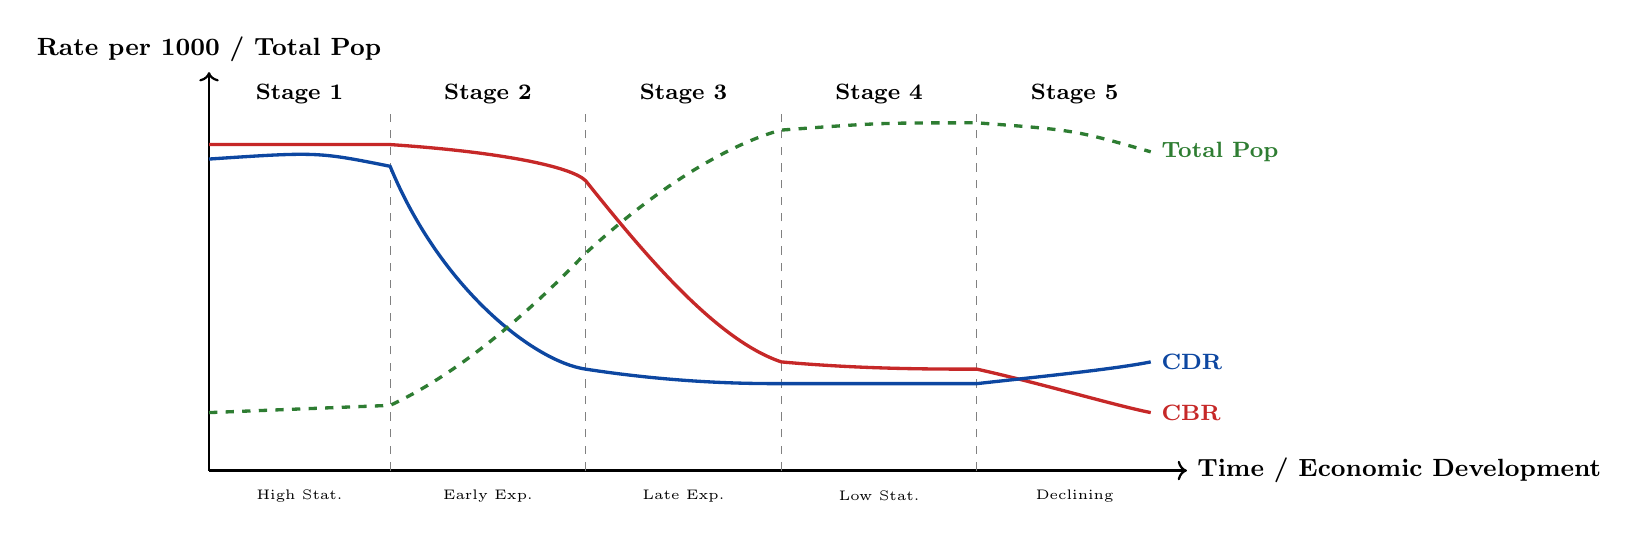
\begin{tikzpicture}[scale=0.92]
  % Axes
  \draw[->, thick] (0,0) -- (13.5,0) node[right] {\small \textbf{Time / Economic Development}};
  \draw[->, thick] (0,0) -- (0,5.5) node[above] {\small \textbf{Rate per 1000 / Total Pop}};
  
  % Stage Division Lines
  \draw[dashed, gray] (2.5,0) -- (2.5,5);
  \draw[dashed, gray] (5.2,0) -- (5.2,5);
  \draw[dashed, gray] (7.9,0) -- (7.9,5);
  \draw[dashed, gray] (10.6,0) -- (10.6,5);
  
  % Stage Labels
  \node at (1.25,5.2) {\footnotesize \textbf{Stage 1}};
  \node at (3.85,5.2) {\footnotesize \textbf{Stage 2}};
  \node at (6.55,5.2) {\footnotesize \textbf{Stage 3}};
  \node at (9.25,5.2) {\footnotesize \textbf{Stage 4}};
  \node at (11.95,5.2) {\footnotesize \textbf{Stage 5}};
  
  \node at (1.25,-0.35) {\tiny High Stat.};
  \node at (3.85,-0.35) {\tiny Early Exp.};
  \node at (6.55,-0.35) {\tiny Late Exp.};
  \node at (9.25,-0.35) {\tiny Low Stat.};
  \node at (11.95,-0.35) {\tiny Declining};

  % CBR Curve (Red)
  \draw[very thick, accentred] 
    (0,4.5) -- (2.5,4.5) 
    .. controls (4,4.4) and (5,4.2) .. (5.2,4.0)
    .. controls (6,3.0) and (7,1.8) .. (7.9,1.5)
    .. controls (9,1.4) and (10,1.4) .. (10.6,1.4)
    .. controls (11.5,1.2) and (12.5,0.9) .. (13,0.8)
    node[right] {\footnotesize \textbf{CBR}};

  % CDR Curve (Blue)
  \draw[very thick, primaryblue] 
    (0,4.3) .. controls (1.5,4.4) .. (2.5,4.2)
    .. controls (3.2,2.5) and (4.5,1.5) .. (5.2,1.4)
    .. controls (6.5,1.2) and (7.5,1.2) .. (7.9,1.2)
    .. controls (9,1.2) and (10,1.2) .. (10.6,1.2)
    .. controls (11.5,1.3) and (12.5,1.4) .. (13,1.5)
    node[right] {\footnotesize \textbf{CDR}};

  % Total Population Curve (Green Dashed)
  \draw[very thick, accentgreen, dashed] 
    (0,0.8) -- (2.5,0.9)
    .. controls (3.8,1.5) and (5,2.8) .. (5.2,3.0)
    .. controls (6.5,4.2) and (7.5,4.6) .. (7.9,4.7)
    .. controls (9.25,4.8) .. (10.6,4.8)
    .. controls (11.95,4.7) .. (13,4.4)
    node[right] {\footnotesize \textbf{Total Pop}};

\end{tikzpicture}
\end{center}

\newpage
\subsection{Migration: Types, Causes, Consequences and Theories}

\begin{defbox}[Migration]
Migration is defined as the physical movement of people across a specified political or administrative boundary to establish a new permanent or semi-permanent residence.
\end{defbox}

\subsubsection{Typology of Migration Streams}
\begin{itemize}[leftmargin=*]
  \item \textbf{By Spatial Boundary}:
  \begin{itemize}
    \item \textit{Internal Migration}: Movement within national borders (Intra-district, Inter-district, Inter-state).
    \item \textit{International Migration}: Movement across national boundaries (Emigration out of a country; Immigration into a country).
  \end{itemize}
  
  \item \textbf{By Directional Stream (Internal)}:
  \begin{enumerate}
    \item \textbf{Rural to Urban (R--U)}: Primary stream driven by industrialization, job search, and urban amenities.
    \item \textbf{Rural to Rural (R--R)}: Dominated by agricultural labor movement and female marriage migration in India.
    \item \textbf{Urban to Urban (U--U)}: Stepwise movement from smaller towns to metro cities for career advancement.
    \item \textbf{Urban to Rural (U--R)}: Counter-urbanization observed among retirees or during crises (e.g., COVID-19 pandemic return migration).
  \end{enumerate}

  \item \textbf{By Volition}:
  \begin{itemize}
    \item \textit{Voluntary Migration}: Based on free personal choice to improve standard of living.
    \item \textit{Forced / Involuntary Migration}: Driven by environmental disasters, warfare, persecution (\textbf{Refugees}, **IDPs**).
  \end{itemize}
\end{itemize}

\subsubsection{Causes of Migration: Push vs. Pull Framework}
\begin{table}[h!]
\centering
\small
\begin{tabularx}{\textwidth}{X X}
\toprule
\textbf{Push Factors (Origin / Negative Drivers)} & \textbf{Pull Factors (Destination / Positive Attractions)} \\
\midrule
High unemployment, low agricultural wages & Abundant job opportunities, higher real wages \\
Land fragmentation, rural poverty, drought/famine & Superior infrastructure, healthcare, education \\
Social discrimination, caste oppression & Social mobility, anonymity, freedom \\
Political instability, civil war, ethnic conflict & Political security, rule of law, safety \\
Environmental degradation, climate displacement & Pleasant climate, urban entertainment \& amenities \\
\bottomrule
\end{tabularx}
\caption{The Push-Pull Matrix Governing Migration Decisions}
\end{table}

\subsubsection{Consequences of Migration}
Migration produces profound demographic, economic, social, and environmental impacts on both origin and destination regions:

\begin{enumerate}[leftmargin=*]
  \item \textbf{Economic Impact}:
  \begin{itemize}
    \item \textit{Origin}: Inflow of \textbf{remittances} (e.g., Kerala model, Bihar rural economy) boosting household consumption and debt payment.
    \item \textit{Destination}: Provides crucial cheap labor for construction, manufacturing, and services, driving urban GDP growth.
  \end{itemize}

  \item \textbf{Demographic Impact}:
  \begin{itemize}
    \item \textit{Origin}: Depleted of young, working-age males, resulting in an aging population and skewed sex ratio (prevalence of females/elderly).
    \item \textit{Destination}: Influx of working-age population alters age-sex pyramids, increasing male proportion in urban hubs.
  \end{itemize}

  \item \textbf{Social \& Cultural Impact}:
  \begin{itemize}
    \item Inter-mixing of cultures, diffusion of new ideas, technologies, and cosmopolitan lifestyles.
    \item Negative: Potential friction, social alienation, and xenophobic reactions from native populations.
  \end{itemize}
\end{enumerate}

\subsubsection{Theories of Migration}
\begin{enumerate}[leftmargin=*]
  \item \textbf{Ravenstein's Laws of Migration (1885)}:
  \begin{itemize}
    \item The majority of migrants travel short distances.
    \item Migration proceeds step-by-step toward major commercial hubs.
    \item Each main migration stream produces a compensating counter-stream.
    \item Urban residents are less migratory than rural residents.
    \item Females predominate in short-distance internal movements; males dominate long-distance international moves.
    \item Economic motives form the primary impulse for migration.
  \end{itemize}

  \item \textbf{Everett Lee's Push-Pull Theory (1966)}:
  \begin{itemize}
    \item Conceptualized migration as governed by 4 factors:
    \begin{enumerate}
      \item Factors associated with the area of origin.
      \item Factors associated with the area of destination.
      \item \textbf{Intervening Obstacles} (distance, cost, physical barriers, migration laws).
      \item Personal factors (age, intelligence, risk tolerance).
    \end{enumerate}
  \end{itemize}
\end{enumerate}

\newpage
\subsection{Rural Settlements in India: Characteristics, Types & Patterns}

\begin{defbox}[Rural Settlement]
A rural settlement is a spatial cluster of human habitations situated in a countryside environment where the majority of residents ($>75\%$) are directly engaged in primary economic activities (agriculture, animal husbandry, fishing, forestry).
\end{defbox}

\subsubsection{Determinants of Rural Settlements in India}
\begin{itemize}[leftmargin=*]
  \item \textbf{Physical Factors}: Water availability (\textbf{Wet-point settlements} near springs/rivers vs. \textbf{Dry-point settlements} built on raised knolls to avoid floods), relief, soil fertility, climate.
  \item \textbf{Cultural / Social Factors}: Caste hierarchy (spatial separation of hamlets based on caste), religion, tribal social organization.
  \item \textbf{Security / Defense Factors}: History of invasions, wild animal threats, leading to fortified compact villages (e.g., Bundelkhand, Nagaland).
\end{itemize}

\subsubsection{Four Types of Rural Settlements in India}
\begin{enumerate}[leftmargin=*]
  \item \textbf{Clustered / Nucleated Settlements}:
  \begin{itemize}
    \item \textit{Morphology}: Houses are tightly built adjacent to one another with narrow, winding lanes. Living area is distinctly separated from surrounding farmland.
    \item \textit{Distribution}: Highly fertile Indo-Gangetic Plains (Punjab, Haryana, UP, Bihar), Rajasthan (water security forces clustering around wells), and Nagaland (defense).
  \end{itemize}

  \item \textbf{Semi-Clustered / Fragmented Settlements}:
  \begin{itemize}
    \item \textit{Morphology}: Results from forced segregation or expansion of a clustered village. Dominant landowning caste occupies the main central nucleus, while lower caste social groups are forced to settle on the outer periphery.
    \item \textit{Distribution}: Gujarat plains, Malwa plateau, parts of Rajasthan.
  \end{itemize}

  \item \textbf{Hamleted Settlements (\textit{Panna, Para, Palli, Nagla, Dhani})}:
  \begin{itemize}
    \item \textit{Morphology}: Settlement is physically divided into several small isolated units dispersed across the village territory, but linked by a common name.
    \item \textit{Distribution}: Middle and lower Gangetic plains, Chhattisgarh, Himalayan valleys.
  \end{itemize}

  \item \textbf{Dispersed / Isolated Settlements}:
  \begin{itemize}
    \item \textit{Morphology}: Isolated homesteads or tiny huts scattered over fields, forest tracts, or hill slopes.
    \item \textit{Distribution}: Meghalaya, Himachal Pradesh, Uttarakhand, Western Ghats, desert dunes of western Rajasthan.
  \end{itemize}
\end{enumerate}

\subsubsection{Geometrical Settlement Patterns}
Rural settlements arrange themselves in distinct geometric shapes based on terrain and transport infrastructure:
\begin{itemize}[leftmargin=*]
  \item \textbf{Linear Pattern}: Houses built along a single linear feature such as a road, railway track, canal bank, or river levee.
  \item \textbf{Rectangular Pattern}: Found in flat alluvial plains and planned agricultural zones where streets intersect at right angles ($90^\circ$).
  \item \textbf{Circular Pattern}: Houses built surrounding a central water body (pond, lake), village green, or temple.
  \item \textbf{Star-Shaped / Radial Pattern}: Develops where multiple transport routes converge; houses extend outward along all radiating roads.
  \item \textbf{T-Shaped / Y-Shaped / Cross-Shaped}: Develops specifically at tri-junctions, river confluences, or crossroads.
\end{itemize}

\newpage
\subsection{Urban Settlements: Evolution, Classification & Morphology}

\subsubsection{Census of India Definition of Urban Area}
According to the Census of India, an \textbf{Urban Settlement} is defined as:
\begin{enumerate}[leftmargin=*]
  \item All places with a Municipality, Corporation, Cantonment Board, or Notified Town Area Committee (**Statutory Town**).
  \item All other places satisfying three criteria simultaneously (**Census Town**):
  \begin{itemize}
    \item Minimum total population of \textbf{5,000}.
    \item At least \textbf{75\% of male main working population} engaged in non-agricultural pursuits.
    \item Density of population of at least \textbf{400 persons per sq. km} (1,000 per sq. mile).
  \end{itemize}
\end{enumerate}

\subsubsection{Functional Classification of Indian Towns}
Based on their primary economic function and administrative role:
\begin{table}[h!]
\centering
\small
\begin{tabularx}{\textwidth}{l X X}
\toprule
\textbf{Functional Category} & \textbf{Primary Economic Activity} & \textbf{Prominent Indian Examples} \\
\midrule
\textbf{Administrative Towns} & National/State capitals, government headquarters & New Delhi, Chandigarh, Bhopal, Dispur \\
\textbf{Industrial Towns} & Heavy manufacturing, steel, textiles, chemicals & Jamshedpur, Bhilai, Kanpur, Rourkela \\
\textbf{Transport / Port Towns} & Maritime trade, major railway junctions, logistics & Mumbai, Kandla, Visakhapatnam, Mughalsarai \\
\textbf{Commercial Towns} & Trade, wholesale markets, financial services & Ahmedabad, Surat, Indore, Ludhiana \\
\textbf{Mining Towns} & Mineral extraction, coalfields, oil fields & Raniganj, Jharia, Singrauli, Digboi \\
\textbf{Garrison / Cantt Towns} & Military headquarters, defense establishments & Ambala, Mhow, Jalandhar Cantt, Pathankot \\
\textbf{Educational Towns} & Universities, research hubs, coaching institutes & Roorkee, Oxford, Varanasi, Kota \\
\textbf{Religious / Cultural} & Pilgrimage centers, historical heritage & Varanasi, Haridwar, Puri, Tirupati, Amritsar \\
\textbf{Tourist / Resort Towns} & Hill stations, coastal resorts, recreation & Shimla, Nainital, Ooty, Darjeeling, Goa \\
\bottomrule
\end{tabularx}
\caption{Functional Classification of Urban Centers in India}
\end{table}

\subsubsection{Classic Theories of Urban Morphology}

\begin{enumerate}[leftmargin=*]
  \item \textbf{Burgess Concentric Zone Model (1925)}:
  \begin{itemize}
    \item Developed by Ernest Burgess observing Chicago. City expands radially outward from a central core in 5 concentric rings:
    \begin{enumerate}
      \item \textit{Zone 1}: Central Business District (CBD / Loop).
      \item \textit{Zone 2}: Zone of Transition (slums, light industry, blighted housing).
      \item \textit{Zone 3}: Zone of Independent Workingmen's Homes (blue-collar housing).
      \item \textit{Zone 4}: Zone of Better Residences (middle-class single-family homes).
      \item \textit{Zone 5}: Commuters' Zone (suburban fringe).
    \end{enumerate}
  \end{itemize}

  \item \textbf{Hoyt Sector Model (1939)}:
  \begin{itemize}
    \item Developed by Homer Hoyt. Argued cities expand not in ring shapes, but in \textbf{wedge-shaped sectors} along major radial transportation corridors (railways, highways). High-rent residential areas grow outward along pleasant high ground, while heavy industry clings to rail lines and waterways.
  \end{itemize}

  \item \textbf{Harris and Ullman Multiple Nuclei Model (1945)}:
  \begin{itemize}
    \item Proposed by Chauncy Harris and Edward Ullman. Asserts that modern large cities do not revolve around a single CBD, but grow around \textbf{multiple independent operational nodes} (e.g., ports, suburban business parks, universities, industrial estates).
  \end{itemize}
\end{enumerate}

\newpage
% ==========================================
% UNIT IV: EXAM REVISION & MODEL ANSWERS
% ==========================================
\section{Unit IV: Exam Quick Revision & Model Answer Outlines}

\begin{exambox}[Model Answer Outline 1: Environmental Determinism vs. Possibilism]
\textbf{Exam Question}: \textit{``Critically analyze Environmental Determinism and Possibilism. How does Griffith Taylor's Neo-Determinism reconcile these opposing philosophies?''} (15 Marks)
\end{exambox}

\subsubsection{Structure for a 15-Mark Model Answer}
\begin{enumerate}[leftmargin=*]
  \item \textbf{Introduction (2 Marks)}:
  \begin{itemize}
    \item Define Human Geography as the study of man-environment interaction.
    \item Introduce the core debate: Determinism (nature dominant) vs. Possibilism (human agency dominant).
  \end{itemize}
  
  \item \textbf{Environmental Determinism (4 Marks)}:
  \begin{itemize}
    \item Define core concept; mention key proponents (Ratzel, Semple, Huntington).
    \item Cite Semple's quote (\textit{``Man is a product of the surface of the earth...''}).
    \item Give examples (climatic control over energy and culture).
    \item Highlight critiques (racial bias, technological ignorance).
  \end{itemize}

  \item \textbf{Possibilism (4 Marks)}:
  \begin{itemize}
    \item Define core concept; mention Febvre, Vidal de la Blache, Carl Sauer.
    \item Explain \textit{Genre de Vie} and cultural landscape.
    \item Cite examples of human adaptation via technology (greenhouses, irrigation).
    \item Highlight critiques (environmental destruction, ecological blindness).
  \end{itemize}

  \item \textbf{Neo-Determinism as a Synthesis (4 Marks)}:
  \begin{itemize}
    \item Introduce Griffith Taylor (1951) and \textit{Stop-and-Go Determinism}.
    \item Explain the \textbf{Traffic Controller Analogy}.
    \item Connect to modern \textbf{Sustainable Development} and ecological planetary boundaries.
  \end{itemize}

  \item \textbf{Conclusion (1 Mark)}:
  \begin{itemize}
    \item Conclude that man and environment are complementary components of a single ecosystem; true development lies in harmony with natural limits.
  \end{itemize}
\end{enumerate}

\begin{exambox}[Model Answer Outline 2: Demographic Transition Theory]
\textbf{Exam Question}: \textit{``Examine the Demographic Transition Theory with the help of a suitable diagram. Discuss its applicability to developing nations like India.''} (15 Marks)
\end{exambox}

\subsubsection{Structure for a 15-Mark Model Answer}
\begin{enumerate}[leftmargin=*]
  \item \textbf{Introduction \& Proponents (2 Marks)}: Mention Thompson (1929) and Notestein (1945). State that DTT models transition from High CBR/CDR to Low CBR/CDR alongside industrialization.
  \item \textbf{Annotated Diagram (3 Marks)}: Draw clear curves for CBR, CDR, and Total Population across 5 distinct stages.
  \item \textbf{Elaboration of Stages (5 Marks)}: Detail CBR, CDR, and NIR characteristics for Stage 1 through Stage 5 with modern country examples.
  \item \textbf{Applicability to India & Developing World (4 Marks)}:
  \begin{itemize}
    \item India entered Stage 2 around 1921 (\textit{Year of Great Divide}) due to mortality decline.
    \item India transitioned to Stage 3 (Late Expanding) post-1981 with falling fertility rates (Total Fertility Rate dropped to $2.0$ in NFHS-5).
    \item Critique: Western DTT assumed natural economic development, whereas developing nations experienced rapid medical-induced mortality drops ahead of economic industrialization.
  \end{itemize}
  \item \textbf{Conclusion (1 Mark)}: Summarize the policy imperative of reaping India's demographic dividend before entering Stage 4 aging.
\end{enumerate}

\end{document}
